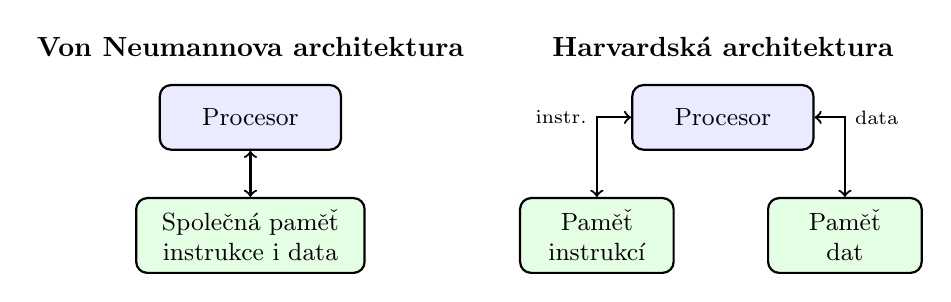
\begin{tikzpicture}[
    x=1cm, y=1cm,
    every node/.style={font=\small},
    title/.style={font=\bfseries},
    unit/.style={
        draw,
        thick,
        rounded corners,
        align=center,
        minimum width=2.25cm,
        minimum height=0.72cm
    },
    arr/.style={<->, thick}
]

    % Left title
    \node[title] at (-3.0, 1.35) {Von Neumannova architektura};

    % Left diagram
    \node[
        unit,
        fill=blue!8,
        minimum width=2.30cm,
        minimum height=0.82cm
    ] (cpuA) at (-3.0, 0.45) {Procesor};

    \node[
        unit,
        fill=green!10,
        minimum width=2.90cm,
        minimum height=0.95cm
    ] (memA) at (-3.0, -1.05) {Společná paměť\\ instrukce i data};

    \draw[arr] (cpuA.south) -- (memA.north);

    % Right title
    \node[title] at (3.0, 1.35) {Harvardská architektura};

    % Right diagram
    \node[
        unit,
        fill=blue!8,
        minimum width=2.30cm,
        minimum height=0.82cm
    ] (cpuB) at (3.0, 0.45) {Procesor};

    \node[
        unit,
        fill=green!10,
        minimum width=1.95cm,
        minimum height=0.95cm
    ] (imem) at (1.40, -1.05) {Paměť\\ instrukcí};

    \node[
        unit,
        fill=green!10,
        minimum width=1.95cm,
        minimum height=0.95cm
    ] (dmem) at (4.55, -1.05) {Paměť\\ dat};

    \draw[arr] (cpuB.west) -| node[left, font=\scriptsize] {instr.} (imem.north);
    \draw[arr] (cpuB.east) -| node[right, font=\scriptsize] {data} (dmem.north);

\end{tikzpicture}
